% NOTE - this is only a template without real arguments
\begin{entry}{Phase 2 completion}{Nov 8, 2021}
    \objective 
    
    Complete, test, and refactor phase 2.


    \outline

    \begin{itemize}
        \item Establish locational association data (EDM topology, node MRIDs most likely)
        \begin{itemize}
            \item https://miro.com/app/board/o9J_luL3bbE=/
        \end{itemize}
        \item Establish DERIdentificationManager
        \item Establish DERAssignmentHandler
        \item Write a test Historical Data input log using locational data
        \item Write DERSHistoricalDataInput locational data function (standard)
        \item Modify MCInputInterface to use DERIdentificationManager association tables by default
        \item Functional asynchronous test of MC: Logs-Assignment-Association-Realtime data-convertion-Input-Sim-Output-Logs
        \item Add association data feedthrough to EDMMeasurementProcessor
        \item Test EDMMeasurementProcessor
        \item Attempt to add 2-phase battery inverters to buses.
    \end{itemize}

    \procedures

    \section*{Establish Topological Processor}
    Topology refers to the location or orientation of components in the model in relation to one another. The most basic
    locational "units" in the model are Buses; each DER-EM is connected to a Bus, and that connection and therefore bus
    would be located somewhere in the world.

    However, the Grid Operator (and any contracted DERMS or GSP) wouldn't necessarily view the grid in terms of
    individual buses. The GSP's server/client program, for instance, expects information in "Groups". These Groups may
    be concerned with one bus, groups of buses, information coming from particular topological branches, etc. This
    topology is something that needs to be decided ahead of time in accordance with the GO's needs; or, in our case,
    with the parameters of the testing we're doing with the GSP.

    To this end, we developed a topological processing class, GOTopologyProcessor. The topology is stored within an
    .xml file, in the repository as "topology.xml". This xml file is used to generate a topology lookup "dictionary",
    with each "Group" key containing a number of "Bus" values. This can be used to determine which buses are within
    a Group, so that the proper data is being provided to the GSP by the GO (later in development). The dictionary
    can be reversed so that each bus can be queried for whatever groups it is in.

    Currently, we're concerned with functional development and testing of our respective systems; so, each Group is
    associated one-to-one to each bus in the 13-node model. Group 1 is Bus 650 only, Group 2 is Bus 646, etc.

    \section*{Establish DERIdentificationManager and DERAssignmentHandler}
    The input to the MC will come from a variety of sources via DER-S classes. One (conceptual) requirement of each
    input is that it needs to be located somewhere in the model; without that locational data, DERs would be assigned
    arbitrarily to buses throughout the model and topology would become meaningless. Each input DER also needs some sort
    of name or unique identifier so that the system can keep track of which data is going to which DER-EM. Finally, the
    DER inputs need "operating data" such as power consumed, importing/exporting, etc; this can be a lot of things, but
    the idea is that it is the data that is being used to determine the updated grid states of each DER.

    Each DER-EM has an mRID associated with it's inputs and controls. This is internal to the CIM model and not known to
    external inputs. What is known is the bus each input will be assigned to. So, it is possible to assign each input
    to a DER-EM mRID on the proper bus automatically, provided a DER-EM exists on that bus. So the first step in the
    assignment development was to automate DER-EM addition.

    \subsubsection*{CIMHub}
    PNNL provides a set of tools and scripts that allow modifications to an existing model in the blazegraph database. 
    IMPORTANT NOTE: fully stopping the docker container with `./stop.sh -c` or an updated version of GridAPPS requires
    the process to be rerun.
    
    These scripts look at a user-generated text file containing a list of all the DERs we want added to the model, 
    their Bus location (by bus name), and label plate information. This text file is used to drop existing DERs, add
    the new DER-EMs, and generate the required mRIDs as well as measurement mRIDs for each. The process by which it 
    does so is beyond the scope of our project; suffice to say that the mRIDs can be easily gleaned by database queries
    either using the web app or within the MC. So, in order to add the proper amount of DER-EMs, we modify the text file
    and run the Initialise_DER_EMs.bat batch script to run all the necessary routines.
    
    This must be accomplished before running the MC simulation (though later on it will likely be integrated with the MC
    via the batch script.) Because of this, we can't simply add DER-EMs dynamically for each input. Ensuring the proper
    number of DER-EMs is added to the text file prior to simulation will need to be part of the test procedure. 
    However, we CAN automate generation of said text file. This is not yet implemented, but the idea is that the GSP
    will generate this text file during its own registration process; it will then be merged with another text file that
    will contain extra DER-EMs as required for the input logs (for instance). This will ensure that there are enough
    DER-EMs on each bus to represent all inputs. If not, the assignment handler throws an exception and closes the
    MC program.
    
    \subsubsection*{DERAssignmentHandler}
    Each DER-S object requires a \verb|self.assign_der_s_to_der_em()| method, which is called
    once by \verb|DERAssignmentHandler.assign_all_ders()| during the MC startup process. This is
    part of the DER-S API function, since each input will represent and provide locational data in different ways. This
    customizable method retrieves the names and associated buses for each input in the DER-S via some custom function,
    uses the Bus to get an mRID for a DER-EM on the proper bus, and associates the name with the mRID. The name and bus
    information are fed through to the measurement processor, which makes the data easier to compare (since measurement
    names use the DER-EM name, while the input names are whatever the input uses.)

    \subsubsection*{DERIdentificationManager}
    This class is a bit more simple; it takes the input name/mRID association data and stores it in a lookup table.
    The accessor methods return an mRID for a given name, or vice versa. This is used by the MCInputInterface; each
    timestep it retrieves updated states from each DER-S and stores them in a unified input request, each line of which
    contains the name and operating states for each DER input this timestep. The MCInputInterface takes the names and
    looks up the proper mRIDs for each, then uses the mRID/data pairs to generate the proper input requests on the
    Simulation API using the gridappsd python library.

    This method thus allows inputs to be delivered to DER-EMs on the proper bus without EVER needing the inputs or
    DER-Ss to know any of the model data. As long as the input is on a valid bus with an available DER-EM, the input
    will be assigned and updated states will be sent properly and automatically.

    \section*{Update input logs and DERHistoricalDataInput}
    The previous "test" functionality used mRID names as log headers to forcefully send updated states to DER-EMs. The
    logs needed to be updated to use a more realistic functionality using names and Bus numbers to utilize the
    Assignment and Identification classes. The logs and DERHistoricalDataInput were iterated on to create a better test
    case as follows.

    \subsection*{Logs}
    The logs were modified by doubling the columns. If the first (Timestamp) column is removed, the columns are paired.
    The first column in each pair contains "data" (in this case, real power consumed) and the second column contains the
    bus number. The headers are a unique identifier, along the lines of "DER1", "DER2", etc. Any unique identifier can
    be used. This input method is not optimized since the Bus numbers are only used once in the first timestep for
    identification, but there's no need to overcomplicate the log input at this point. We're just using it for testing
    purposes and this was easy to implement.

    \subsection*{DERHistoricalDataInput}
    The biggest addition to this object was the \verb|.assign_der_s_to_der_em()| method. This
    method goes through the list of DERs read from the (odd) headers in the log file, gets the bus numbers for each
    DER from the even columns of the first line of the .csv, and uses those name/number pairs in the Assignment
    handler to generate the association table (name/mRID). All updates to the class are in service of this function.
    Then each timestep, as before, the class checks to see if there's a line of data corresponding to the current
    simulation timestep, reads the line of data, organizes it into name/value pairs, and sends those name/value pairs
    to the Input Processor, which replaces the name with an mRID (see Identification Manager) and generates the input
    request difference messages.

    \section*{Modify MCInputInterface}
    As has been detailed above, the input branch was modified to assign DER-EM mRIDs to DER inputs by looking up
    DER-EMs available on the proper bus and associating them with input names. The updated states come from the inputs
    in name/value pairs, with the name being a unique itentifier and the value being a power consumption. Association
    data between mRIDs and unique identifiers is handled in the simulation startup by assignment, and used during the
    simulation by looking up mRIDs for a name using the association tables in the Identification Manager. As such, the
    biggest modification to the Input Interface was to add a step in which the Interface reads an input request from a
    DER-S, takes the names, looks up the associated mRIDs using the Identification Manager, and proceeds to generate
    the input request messages GridAPPS-D needs in the proper format (using the difference builder method in the
    gridappsd library; unchanged from Phase 1)

    \textit{One important note is that power consumption (and presumably generation) is the ONLY implemented grid
    state input right now. Any other usage of the DER-EMs (voltage or reactive power, for instance) will require
    additional methods in the MCInputInterface AS WELL AS an iteration on the input request message format between
    the DER-S and Input Interface. This iteration will need to include a key/value pair for type of grid state
    update; power, voltage, etc. This will not require any modifications to the assignment or association objects as
    those merely tie names to mRIDs, so it's not expected that this will be a challenge. It's just not yet been
    necessary to implement.}

    \section*{Add association feedthrough data}
    This turned out to be a major pain, but worked in the end. One major challenge of appending association data to
    measurements is that there are multiple mRIDs corresponding to a single component in the model: each DER-EM has
    terminal mRIDs, power connection mRIDs, measurement mRIDs, etc. We needed a way to associate the input mRID with
    the measurement mRID of each DER-EM.

    First, we needed to query GridAPPS-D for a new model dictionary containing all of the possible information for all
    the loads on our feeder model. This was added to \verb|edmCore.establish_mrid_name_lookup_table()|.
    Now instead of just getting the mrid/name lookup table used by the measurement processor, it also
    gets this \verb|"cim_dict".|

    The \verb|cim_dict| is then used in a method in the \verb|EDMMeasurementProcessor.append_names()| and
    \verb|.append_association_data|. The methodology is sloppy and difficult to explain, let alone understand,
    but in short it takes values from both dictionaries and uses it to determine the name of objects based on the
    names of the DER-EMs taken from the \verb|cim_dict.|
    These names need to be parsed and excess characters removed to align data in the
    \verb|cim_dict| with the input association data. Once that's done, we have
    inputName/inputmRID/DER-EMname/measurementmRID data all lumped together, which is then added to each
    measurement's value dictionary each timestep. The end result is that our output logs are MUCH larger, as each
    cell is a dictionary with a half dozen or so key/value pairs. This is obviously not the most efficient method of
    maintaining this data, but as it's all present it will suffice for now. It was always the intent that a set of
    tools would be needed to be developed to unpack and use the logs for analysis, and now the logs are larger but
    much more useful.

    This feedthrough data will also be necessary when the GO is implemented, so feedback can be presented to the DERMS
    about whether DERs are operating as necessary for the dispatch.

    \section*{2-phase DER-EM test}
    In short: this works fine. The 13-node feeder has some 2-phase and 1 phase buses. Using the DER-EM addition script
    and modifications to the text file to use only BC phases (for instance, see above) inverters can be added that only
    use and affect two or even one phase of the grid at that bus. This can be used directly right now; however, there
    is no method to distinguise whether or not a DER-EM is 3 phases or not right now, so that will have to be
    implemented before we can mix 2-phase and 3-phase DER-EMs on the same bus.

    \parameters
    
    N/A

    \observations

    I've done some refactoring, but more can be done. It's just not really worth the time right now. A big thing would
    be cleaning up the appendage stuff in the Measurement Processor.

    I added a new class and object to the system: MCConfiguration. It's mostly a data holding structure for various MC
    config stuff. For example, instead of having to add a method for each DER-S to the startup methods like assignment
    and to the on-timestep DER-S read methods, there is now a single attribute where you can list all active DER-S
    objects and comment out ones that aren't needed.

    Functional testing completed sat. I tried phase 2 testing before implementing the feedthrough, which doesn't work
    becuase a lot of the test plans needed the feedthrough data in the logs to be completed. So in this case I will
    not provide a list of Test Plans completed. They've been updated in their individual documents.


    \data

    Most of the relevent data can be found in the logs. The DER addition scripts are added to a folder called
    /DERScripts, and invoked by the \verb|Initialise_DER_EMs.bat| script.
    Refer to the GitHub repository for more info.

    The individual dictionaries communicated from actor to actor are manipulated using complex and often repetitious
    methods. To see the contents of a dictionary at a given simulation time, the best way to go about it is to add
    a print() function to the code and read it in the terminal.

    \results
    
    All tests completed sat. Phase 2 of the ME is now complete.


\end{entry}


%\begin{entry}{CMake Error running EGOT-DCM Dockerfile}{Dec 02, 2020}
%    \objective
%
%    Determine the cause of the CMake error while running the dockerfile and modify file to get it to successfully build.
%
%    \outline
%
%    \begin{itemize}
%        \item Try running to see if it was just Lorry or a machine issue.
%        \item If it is a machine issue, modify configurations to ensure interoperability.
%        \item If I get the error track down its cause and modify dockerfile to fix.
%        \item Repeat until all builds are successful.
%    \end{itemize}
%
%    \procedures
%
%    \begin{itemize}
%        \item \mint{console}|git clone https://github.com/EGoT-DCS-SunSpec-Modbus|
%        \item \mint{console}|docker build -f Dockerfile.buster -t egot-dcs .|
%        \item \mint{console}|docker container run -i egot-dcs|
%    \end{itemize}
%
%    \observations
%
%    \begin{error}{Cmake Error: No CMAKE\_CXX\_COMPILER found}
%        \begin{figure}[H]
%            \centering
%            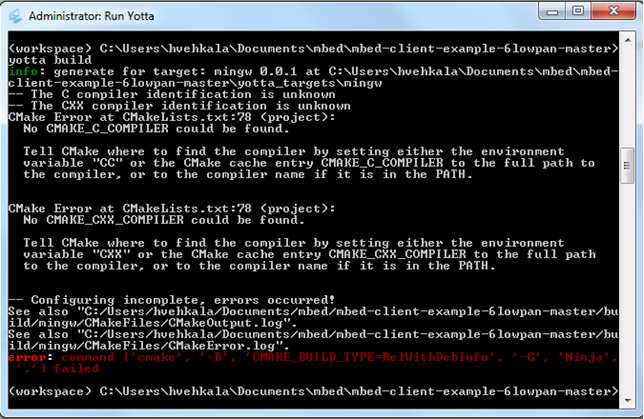
\includegraphics[height=4in]{Fall2020/Figures/cmake_error.png}
%        \end{figure}
%
%        Solution: what you need to do found at \cite{CMAKE-Forum}
%    \end{error}
%
%    \results
%
%    Short: No.
%
%    Long: Well...
%
%
%\end{entry}